% BBC POSE Results
\begin{table}[t]
	\caption{{
	Performance of landmark prediction on BBC Pose test set. As upper bound, we also report the performance of supervised methods.
	%Comparing against supervised and unsupervised methods for annotated landmark prediction on the BBC Pose testing set.
	The metric is \% of points within 6 pixels of groundtruth location. %Note that Jakab et al. are using a 50-landmarks, while we only use a 30 landmarks as input for the regression.
	}}
	\label{tab:bbcpose}
	\centering
	\begin{tabular}{ll|cr}
	\hline
	BBC Pose &   &    { Accuracy}  \\
	 \hline
	supervised & Charles \cite{Charles:2013tb} &
	   79.9\%  \\ % 79.90
	 & Pfister \cite{Pfister:2015uo}  &
	  88.0\%  \\ \hline % 88.01
	unsupervised &Jakab \cite{Jakab:2018wc} &
	 68.4\%  \\  % 68.44
	  &Ours &  \textbf{74.5}\% \\
	% test pck = 0.7484605918670523
	% test pck_per_kp = [0.9633621  0.6627155  0.76508623 0.54956895 0.6928879  0.76616377   0.83943963]
	\hline
	\end{tabular}
\end{table}
%
% HUMAN3.6M Results
\begin{table}[t]
	\caption{{Comparing against supervised, semi-supervised and unsupervised methods for landmark prediction on the Human3.6M test set. The
	error is in \% of the edge length of the image. All methods predict 16 landmarks.
	}}
	\label{tab:human}
	\centering
	\begin{tabular}{ll|cr}
	\hline
	 Human3.6M   & &  { Error w.r.t. image size}  \\
	 \hline
	 supervised & Newell \cite{Newell:2016vq}
	  &2.16  \\  \hline
	 semi-supervised & Zhang \cite{Zhang:2018vz}
	  & 4.14  \\ \hline
	 unsupervised & Thewlis \cite{Thewlis:2017wi}
	 & 7.51  \\
	  & Zhang \cite{Zhang:2018vz}
		& 4.91 \\
	  & Ours& \textbf{2.79} \\
	\hline
	\end{tabular}
\end{table}
% SHOW DISENTANGLING: SHAPE
%\begin{figure}[t]
%	\begin{subfigure}{0.5\textwidth}
%	\centering
%	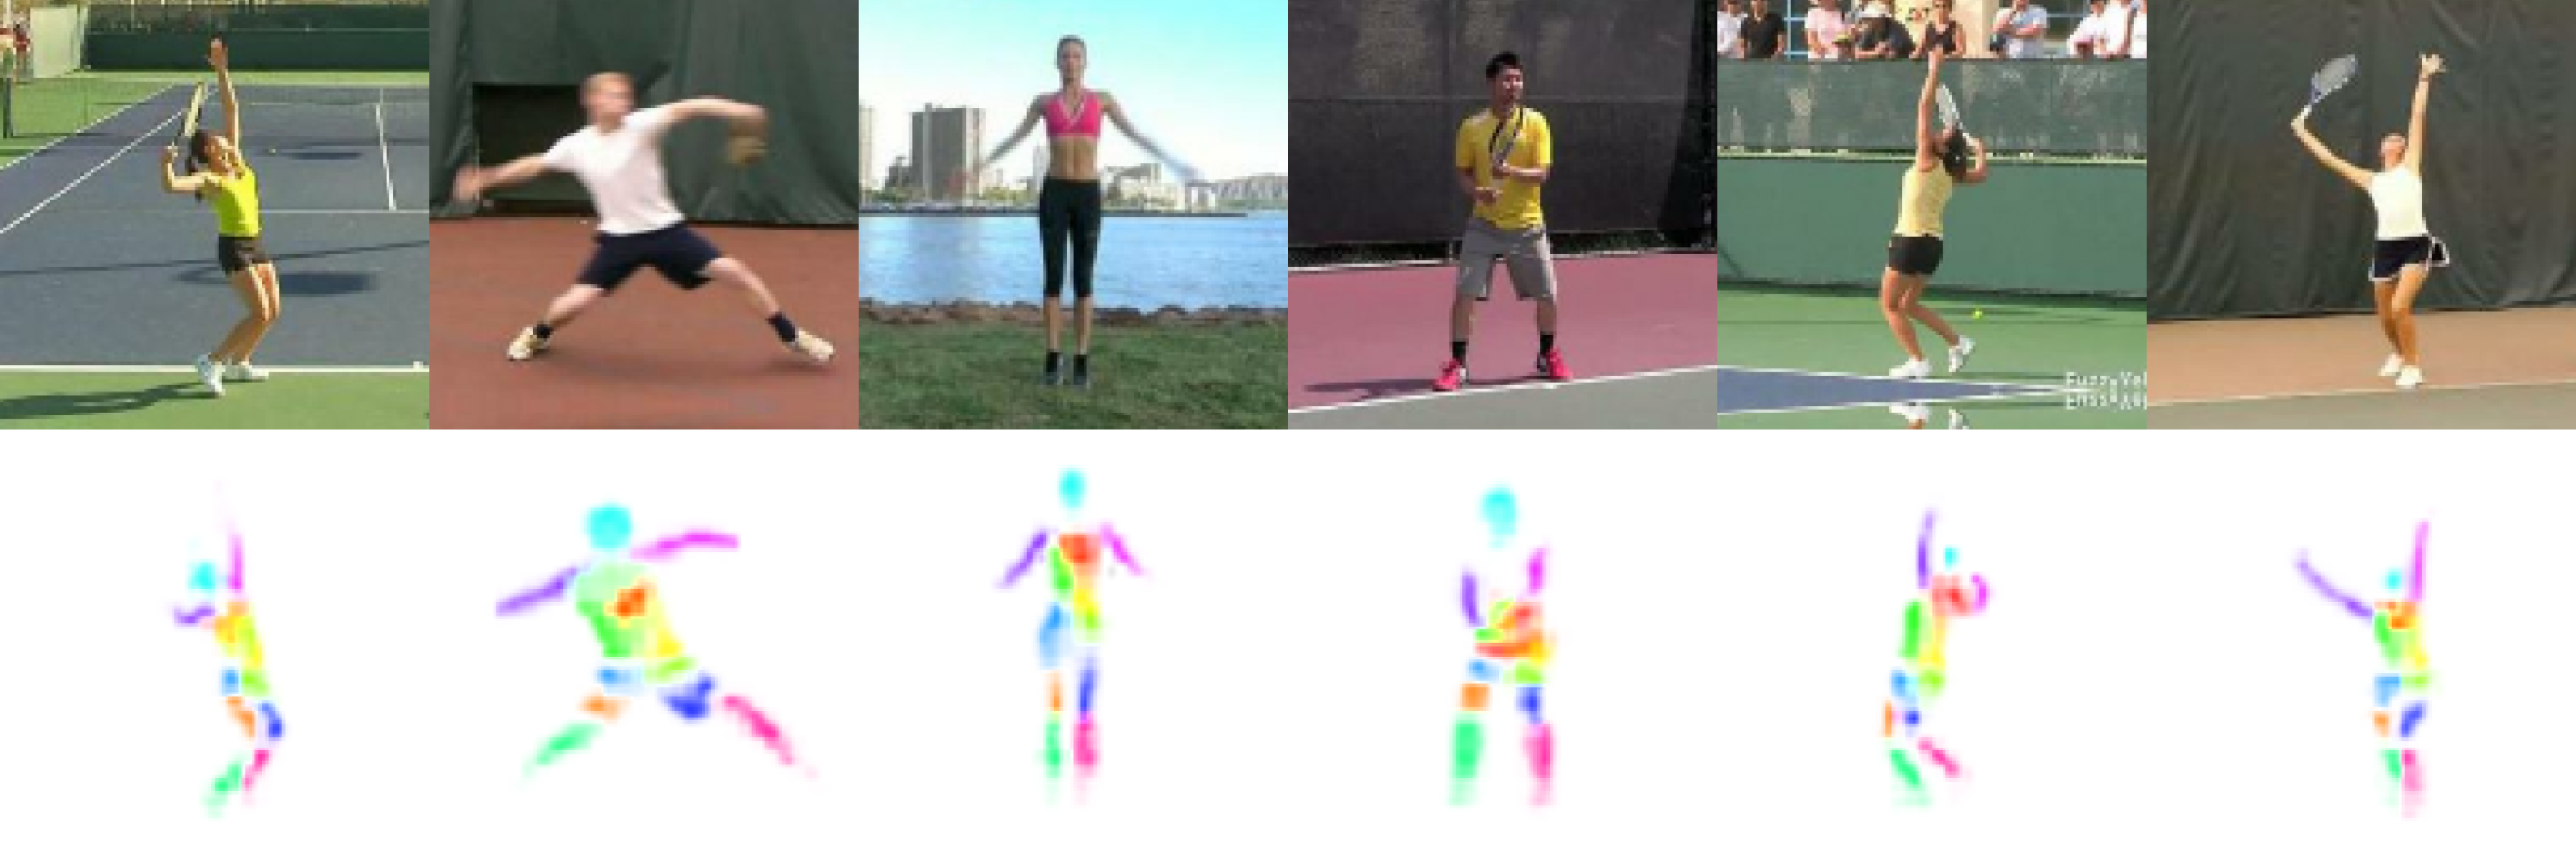
\includegraphics[trim={0cm 0cm 0cm 0cm},clip, width=1.\linewidth]{mat/shape6white}\caption{}
%	\label{fig:shape_penn}
%	\end{subfigure}
%	\begin{subfigure}{0.5\textwidth}
%	\centering
%	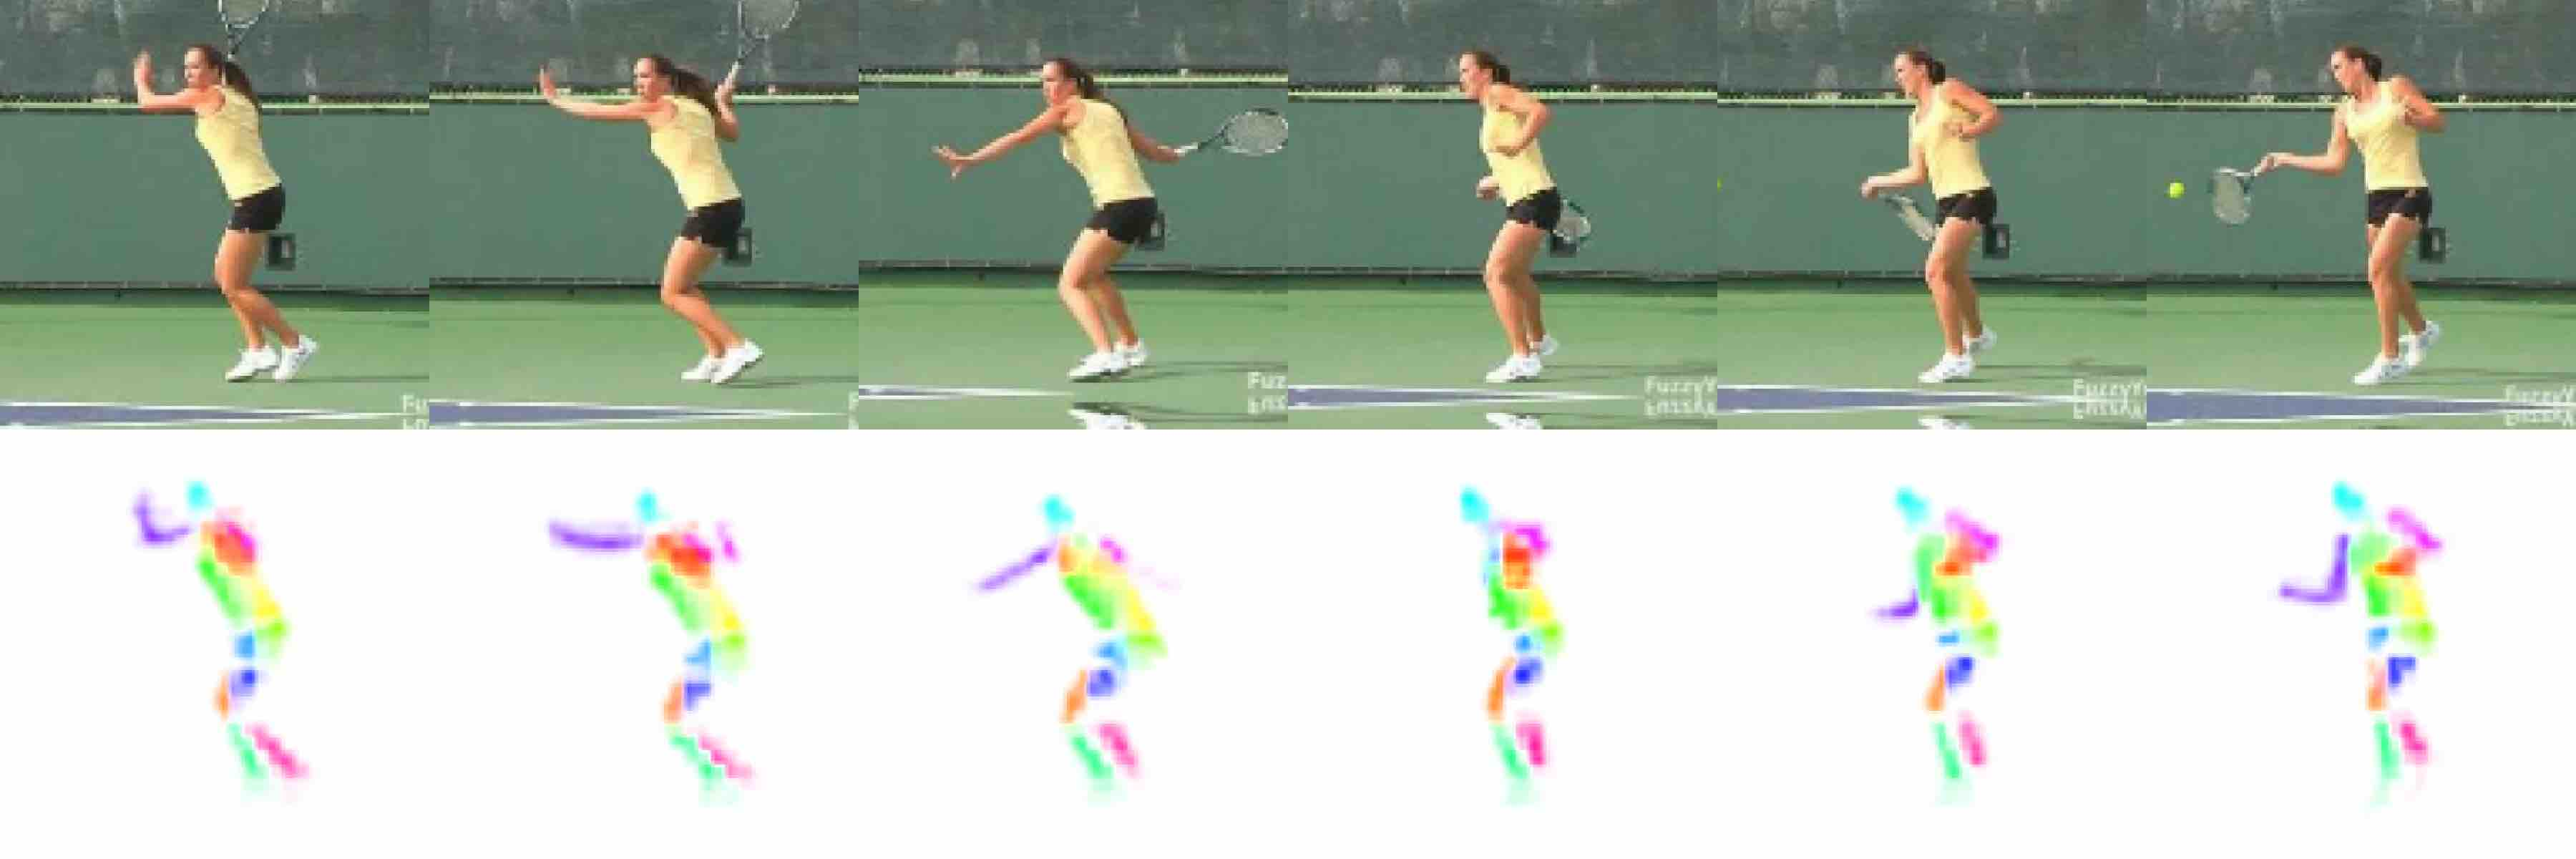
\includegraphics[trim={0cm 0cm 0cm 0cm},clip, width=1.\linewidth]{mat/shape_tennis}\caption{}
%	\label{fig:shape_tennis}
%	\end{subfigure}
	%\begin{subfigure}{0.5\textwidth}
	%\centering
	%\includegraphics[trim={0cm 0cm 0cm 0cm},clip, width=1.\linewidth]{mat/shape_yoga}\caption{}
	%\label{fig:shape_yoga}
	%\end{subfigure}
%	\caption{{Extracting shape representation on Penn Action, for visualization all part shapes are plotted in one image. (a) Different instances, showing intra-class consistency and a (b) time sequence, showing consistency and smoothness across motion. For more examples please refer to the supplementary.}}
%	\label{fig:shape}
%\end{figure}
